% HiRe-MoMa system overview (README: system.png).
% Build: pdflatex system.tex  (TikZ only, no standalone class needed); system.png = system.pdf at 220 dpi.
\documentclass{article}
\usepackage[T1]{fontenc}
\usepackage{lmodern}
\usepackage[scaled=0.95]{helvet}
\renewcommand{\familydefault}{\sfdefault}
\usepackage{sansmath}
\usepackage{tikz}
\usetikzlibrary{fit,backgrounds,arrows.meta,shapes.geometric,calc}

\definecolor{robbg}{HTML}{EAF5E2}  \definecolor{robln}{HTML}{8CC26F}
\definecolor{actbg}{HTML}{F9E9ED}  \definecolor{actln}{HTML}{D79AA9}
\definecolor{lrnbg}{HTML}{E7EEF8}  \definecolor{lrnln}{HTML}{7BA3D3}
\definecolor{boxln}{HTML}{A0A0A0}  \definecolor{arr}{HTML}{454545}

\tikzset{
  box/.style={draw=boxln, fill=white, rounded corners=3pt, line width=0.6pt, align=center,
              minimum height=12.5mm, inner sep=2pt, font=\normalsize},
  db/.style={cylinder, shape border rotate=90, aspect=0.2, draw=lrnln, fill=white, line width=0.7pt,
             minimum width=22mm, minimum height=11.5mm, align=center, font=\footnotesize},
  group/.style={rounded corners=6pt, line width=0.9pt, inner sep=8pt},
  title/.style={font=\bfseries\normalsize, anchor=south west, inner sep=2pt},
  flow/.style={-{Stealth[length=2.4mm]}, line width=0.8pt, draw=arr},
  both/.style={flow, {Stealth[length=2.4mm]}-{Stealth[length=2.4mm]}},
  lbl/.style={font=\footnotesize, text=black!80, align=center, inner sep=1.5pt},
  note/.style={lbl, text=black!60},
}
\newcommand{\sub}[1]{{\footnotesize\color{black!65}#1}}
\newcommand{\code}[1]{{\ttfamily\mdseries #1}}

\newsavebox{\fig}
\newlength{\bd}\setlength{\bd}{6pt}
\begin{document}
\sansmath
\begin{lrbox}{\fig}
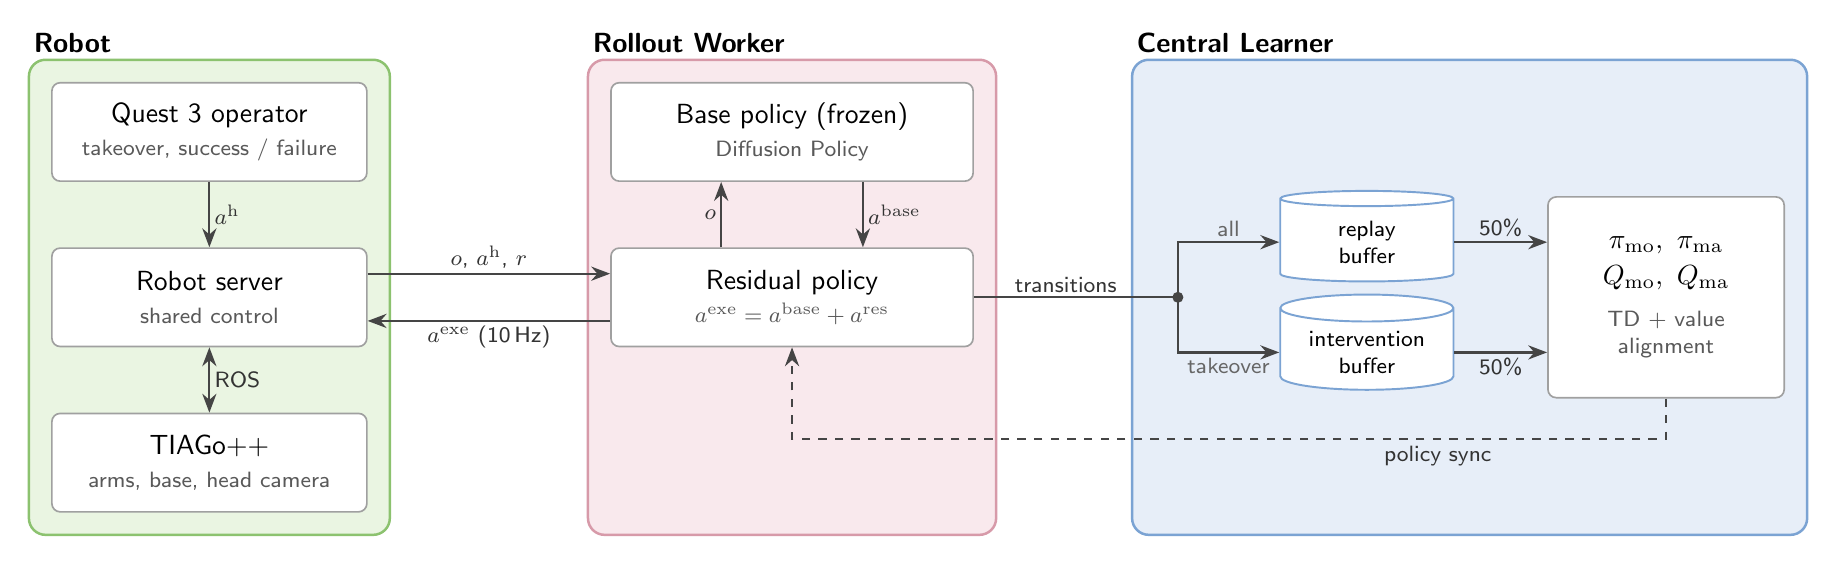
\begin{tikzpicture}[x=1mm, y=1mm]
  % rows: top 0, middle -21, bottom -42
  % ---------------- robot
  \node[box, minimum width=40mm] (vr)    at (20,   0) {Quest 3 operator\\\sub{takeover, success / failure}};
  \node[box, minimum width=40mm] (srv)   at (20, -21) {Robot server\\\sub{shared control}};
  \node[box, minimum width=40mm] (robot) at (20, -42) {TIAGo++\\\sub{arms, base, head camera}};
  \draw[flow] (vr) -- node[lbl, right] {$a^{\mathrm{h}}$} (srv);
  \draw[both] (srv) -- node[lbl, right] {ROS} (robot);

  % ---------------- rollout worker
  \node[box, minimum width=46mm] (dp)    at (94,   0) {Base policy (frozen)\\\sub{Diffusion Policy}};
  \node[box, minimum width=46mm] (actor) at (94, -21) {Residual policy\\\sub{$a^{\mathrm{exe}} = a^{\mathrm{base}} + a^{\mathrm{res}}$}};
  \draw[flow] ([xshift=-9mm]actor.north) -- node[lbl, left]  {$o$} ([xshift=-9mm]dp.south);
  \draw[flow] ([xshift=9mm]dp.south)     -- node[lbl, right] {$a^{\mathrm{base}}$} ([xshift=9mm]actor.north);

  % ---------------- central learner
  \node[db] (auto) at (167, -14) {replay\\buffer};
  \node[db] (intv) at (167, -28) {intervention\\buffer};
  \node[box, minimum width=30mm, minimum height=25.5mm] (heads) at (205, -21)
       {$\pi_{\mathrm{mo}},\ \pi_{\mathrm{ma}}$\\[1pt]$Q_{\mathrm{mo}},\ Q_{\mathrm{ma}}$\\[3pt]\sub{TD + value}\\[-2pt]\sub{alignment}};
  \draw[flow] (auto.east) -- node[lbl, above] {50\%} (heads.west |- auto.east);
  \draw[flow] (intv.east) -- node[lbl, below] {50\%} (heads.west |- intv.east);

  % ---------------- frames (equal heights)
  \coordinate (lrnleft) at (140, -21);
  \begin{scope}[on background layer]
    \node[group, draw=robln, fill=robbg, fit=(vr)(robot)] (G1) {};
    \node[group, draw=actln, fill=actbg, fit=(dp)(actor)(robot.south -| actor)] (G2) {};
    \node[group, draw=lrnln, fill=lrnbg, fit=(heads)(lrnleft)(vr.north -| heads)(robot.south -| heads)] (G3) {};
  \end{scope}
  \node[title] at (G1.north west) {Robot};
  \node[title] at (G2.north west) {Rollout Worker};
  \node[title] at (G3.north west) {Central Learner};

  % ---------------- robot <-> rollout (HTTP), rollout <-> learner (agentlace)
  \draw[flow] ([yshift=3mm]srv.east)    -- node[lbl, above] {$o$, $a^{\mathrm{h}}$, $r$} ([yshift=3mm]actor.west);
  \draw[flow] ([yshift=-3mm]actor.west) -- node[lbl, below] {$a^{\mathrm{exe}}$ (10\,Hz)} ([yshift=-3mm]srv.east);
  \coordinate (split) at (143, -21);
  \draw[line width=0.8pt, draw=arr] (actor.east) -- node[lbl, above, pos=0.45] {transitions} (split);
  \fill[arr] (split) circle (0.7);
  \draw[flow] (split) |- node[note, above, pos=0.75] {all} (auto.west);        % labels centred on the
  \draw[flow] (split) |- node[note, below, pos=0.75] {takeover} (intv.west);   % two branch segments
  \draw[flow, dashed] (heads.south) |- (94, -39) -- (actor.south);
  \node[lbl, anchor=north] at (176, -39.3) {policy sync};
\end{tikzpicture}
\end{lrbox}
\pdfpagewidth=\dimexpr\wd\fig+2\bd\relax
\pdfpageheight=\dimexpr\ht\fig+\dp\fig+2\bd\relax
\hoffset=-1in \voffset=-1in
\shipout\vbox{\kern\bd\hbox{\kern\bd\usebox{\fig}}}
\end{document}
